\chapter{Assembling Panels into a Paper Figure}
\usetikzlibrary{patterns}
\providecommand{\ding}[1]{$\times$}
\providecommand{\sout}[1]{\leavevmode\begingroup\sbox0{#1}\hbox{\copy0\kern-\wd0\rule[0.5ex]{\wd0}{0.4pt}}\endgroup}

Zhou, a doctoral candidate in materials science, is preparing a manuscript on interface passivation in planar perovskite solar cells. On her laptop sit four standalone graphics finished over the past two weeks: a cross-sectional device schematic showing the seven-layer stack, a cross-sectional morphology illustration depicting the vertical grain structure, a current density--voltage ($J\text{--}V$) plot comparing control and passivated devices, and an operational stability plot tracking normalized power conversion efficiency (PCE) under continuous illumination. Needing to assemble Figure 2 before a morning meeting, she drags the four files into a presentation slide in folder order, pulls their corner handles to fill a two-by-two grid, exports the slide as an image, and emails it to her advisor.

The next morning, her manuscript returns with three margin notes on Figure 2: ``Between the blue curve on the bottom left and the red curve on the bottom right, which one is the control?'' ``Did panel b get squashed vertically?'' ``Once shrunk to journal page width, can anyone still read the axis numbers on the bottom left?''

Prompted by those questions, Zhou prints the composite image at 100\% of a standard double-column journal width ($174\ \text{mm}$) on an A4 sheet and inspects it with a ruler. The printout reveals far more than the three issues her advisor flagged. The four panel labels mix three incompatible conventions---an uppercase serif ``A,'' a parenthesized ``(b)'' nearly lost against a dark background, and a lowercase ``c.'' with a period---while the fourth panel has no letter at all. Because the $J\text{--}V$ chart was exported at a large default canvas size and scaled down to fit its cell, its tick labels have shrunk to roughly $4.5\ \text{pt}$, whereas the adjacent stability chart sits at $8\ \text{pt}$. Both data plots use conflicting color palettes and draw both experimental groups as solid lines, making them impossible to tell apart on a monochrome laser printout. Worse still, the horizontal axes of the two side-by-side data panels miss alignment by more than three millimeters.

A multi-panel paper figure is not a storage bin for four separate files; it is a unified visual argument constructed around a single scientific question. Starting from Zhou's returned draft, this chapter walks through how to formulate the overarching question and assign each panel an argumentative role, how to plan a grid at final print dimensions, how to make panels from different tools speak one visual language, and how to align axis spine boxes, panel letters, and whitespace. We then trace the complete reconstruction of the perovskite solar cell Figure 2 and show how to combine deterministic plotting scripts with the multi-panel layout workspace and legend assistant in \scidraw{} to produce a verifiable, review-ready composite figure.

\section{One question, several panels}

Before opening a layout program or drawing a grid, an author needs to answer a foundational question: why do these particular graphics belong together inside one composite figure (Figure 2) rather than standing alone as Figures 2, 3, 4, and 5?

In scholarly publishing, there is only one legitimate reason to combine multiple panels into a single figure: \textbf{the panels jointly answer one higher-level scientific question, and the reader needs to cross-reference evidence across panels within a single field of view} (Rougier et al., 2014; Jambor et al., 2021). When panels address unrelated topics, forcing them onto one canvas fragments the reader's attention. Conversely, when distinct pieces of evidence form a tightly coupled chain of reasoning, placing them on a single double-column spread allows a reviewer to complete an entire analytical loop---understanding the structural modification, checking cross-sectional layer continuity, evaluating initial photovoltaic performance, and verifying long-term operational stability---without flipping pages.

When researchers assemble composite figures without an explicit argumentative plan, they routinely fall into three structural traps:
\begin{itemize}
\item \textbf{Compiling a chronological lab diary:} Ordering panels strictly by the sequence in which instruments were booked---placing early synthesis checks first and device tests last---produces a collage with no central thesis. A reader can study eight panels and still not know what the section is trying to prove.
\item \textbf{Repeating the same claim across redundant panels:} Dedicating two or three separate panels to highly overlapping plots of the same efficiency gain wastes journal space and starves the remaining panels of the area needed for legible typography.
\item \textbf{Crowding routine quality-control checks into the main figure:} Out of anxiety that reviewers might question experimental workload, authors often pack every baseline phase-confirmation spectrum into the main composite figure. Each panel shrinks to postage-stamp size, obscuring fine features of the primary data traces.
\end{itemize}

The antidote to all three traps is to write down the \textbf{main question} of the composite figure in a single testable sentence before touching any graphics software, and then assign each candidate panel a specific \textbf{sub-question and evidential role}. In our perovskite solar cell case study, Figure 2 is built to answer one clear question:

\begin{BookNote}
\textbf{Main question for Figure 2:} Does introducing a passivation layer at the perovskite/hole-transport-layer interface simultaneously improve both the initial power conversion efficiency and the operational stability of planar devices?
\end{BookNote}

Once this overarching question is fixed, the four panels on Zhou's desk acquire distinct, non-overlapping responsibilities in the argument (Figure~\ref{fig:ch09-01}):
\begin{itemize}
\item \textbf{Panel a (device structure schematic):} Answers ``What was modified?'' It establishes the seven-layer planar n-i-p architecture from bottom to top (glass / FTO / $\text{SnO}_2$ / perovskite / passivation layer / spiro-OMeTAD / Au) alongside the direction of incident light, highlighting the exact buried interface where the passivation treatment is introduced. Its evidential role is \textbf{conceptual and explanatory}.
\item \textbf{Panel b (cross-sectional morphology illustration):} Answers ``Are the functional layers continuous, and how does the vertical morphology correspond to the schematic stack?'' It bridges the abstract layer diagram on the left and the physical film stack (in this teaching case, we use a clearly labeled model-generated cross-sectional illustration for layout instruction; in an empirical paper, this slot holds an actual cross-sectional scanning electron micrograph from the same batch of devices).
\item \textbf{Panel c ($J\text{--}V$ characteristic curves):} Answers ``Did initial photovoltaic efficiency improve, and which parameter---open-circuit voltage ($V_{\text{oc}}$), short-circuit current density ($J_{\text{sc}}$), or fill factor (FF)---drove the change?'' Its role is to provide \textbf{quantitative performance evidence}.
\item \textbf{Panel d (normalized PCE over time):} Answers ``Does the interface modification improve long-term operational stability under continuous illumination, and by how much does it extend the time required for efficiency to drop to 80\% of its initial value ($T_{80}$)?'' Its role is to provide \textbf{quantitative durability evidence}.
\end{itemize}

\begin{figure}[htbp]\centering
\resizebox{\linewidth}{!}{% FIG ch09-01 panel argument map (English)
\begin{tikzpicture}[
  x=1mm, y=1mm,
  font=\sffamily\small,
  text=BookInk,
  mainbox/.style={
    draw=BookTeal, line width=0.6pt, rounded corners=2pt,
    fill=BookPale, align=center, text width=150mm, inner sep=3mm,
  },
  explain/.style={
    draw=BookRule, fill=BookRule!35, rounded corners=2pt,
    align=left, text width=38mm, inner sep=2.5mm, minimum height=18mm,
  },
  moved/.style={
    draw=BookInk!40, dashed, rounded corners=2pt,
    align=left, text width=155mm, inner sep=2.5mm,
  },
]
  \node[mainbox] (q) at (87, 58)
    {Main question: does interface passivation raise both initial efficiency and operational stability?};
  \foreach \i/\x/\t in {
    a/20/schematic, b/62/morphology, c/104/performance, d/146/stability} {
    \node[explain] (\i) at (\x, 32) {
      \textbf{\i}\par
      Answers: what changed / layer continuity / initial efficiency / stability over time\par
      \scriptsize Evidence: \t
    };
  }
  \draw[-{Stealth[length=2mm]}, BookInk!60, thick] (q.south) -- (a.north);
  \draw[-{Stealth[length=2mm]}, BookInk!60] (a.east) -- (b.west);
  \draw[-{Stealth[length=2mm]}, BookInk!60] (b.east) -- (c.west);
  \draw[-{Stealth[length=2mm]}, BookInk!60] (c.east) -- (d.west);
  \node[moved] at (87, 8) {
    Candidate moved out (\textbf{example}): XRD pattern $\rightarrow$ Supplementary Information (does not serve the main question)
  };
\end{tikzpicture}
}
\caption{How the panels of Figure 2 share the argument. Each panel answers one sub-question of the main question; a candidate panel that does not serve the main question moves to the Supplementary Information.}\label{fig:ch09-01}
\end{figure}

Defining each panel's role immediately settles the layout sequence: \textbf{reading order must mirror argumentative order}. Readers of scientific journals scan multi-panel figures from left to right and from top to bottom (Jambor et al., 2021). Placing the two explanatory panels (\textbf{a} and \textbf{b}) across the top row to establish ``what the device is,'' and placing the two quantitative data panels (\textbf{c} and \textbf{d}) across the bottom row to demonstrate ``how the device performs,'' creates a natural visual path. As the reader's eye moves along $\textbf{a} \rightarrow \textbf{b} \rightarrow \textbf{c} \rightarrow \textbf{d}$, it follows the exact logical progression from structural design to layer morphology, initial efficiency, and long-term stability, without backtracking across the page.

An explicit argument map also gives a clear criterion for pruning clutter: \textbf{any candidate panel that does not directly advance the main question belongs in the Supplementary Information}. The test is simple: \textbf{If we remove this panel, can Figure 2 still answer its main question completely?} As shown by the dashed box at the bottom of Figure~\ref{fig:ch09-01}, suppose the author also has an X-ray diffraction (XRD) pattern confirming that the annealed film crystallized into the expected perovskite phase without impurity peaks (shown here purely as a planning example; our simulated dataset contains no XRD data). That spectrum answers ``Did the film form the target crystal phase?''---a routine synthesis check rather than direct evidence of whether interface passivation raises efficiency and lifetime. Moving the XRD pattern to the Supplementary Information frees up space so the four core panels remain legible.

At this stage, an author can send the main question and candidate panel list to an AI assistant to help structure sub-questions and flag off-topic panels:

\begin{Prompt}
I am planning Figure 2 (double-column width, 174 mm) for a perovskite solar cell paper.
Main question: Does passivation at the perovskite/hole-transport-layer interface
simultaneously improve initial efficiency and operational stability?
Candidate panels: (1) layered device schematic; (2) cross-sectional morphology image;
(3) control vs. modified J-V curves; (4) 1000 h normalized PCE stability curves;
(5) thin-film XRD phase-confirmation pattern.
List the sub-question and evidence type for each panel, identify which candidate does
not directly serve the main question and should move to Supplementary Information, and
propose a left-to-right, top-to-bottom reading order for the remaining panels.
\end{Prompt}

AI can quickly organize candidate roles from your prompt and point out that item (5) addresses baseline phase purity rather than the interface passivation claim. Yet the boundary of responsibility remains strict: \textbf{AI cannot judge whether your experimental evidence is scientifically sufficient, nor can it decide which measurements may be ethically omitted}. Deciding which results belong in the main text and which routine characterizations move to the supplement rests entirely with the authors.

\section{Plan the grid at final size}

Once the panel roster and reading sequence are locked, the second step is to design the layout grid directly at the \textbf{final print dimensions of the target journal}, rather than plotting individual charts at large default sizes and shrinking them later to fit a multi-panel canvas.

Why is ``plotting big and shrinking later'' the primary cause of illegible text in composite figures? Consider the arithmetic. When you open Python's Matplotlib without specifying dimensions, the default canvas is $8 \times 6\ \text{in}$ ($203.2 \times 152.4\ \text{mm}$) with $10\ \text{pt}$ text. Viewed alone on a laptop screen, that chart looks well proportioned. In print and PDF layouts, however, journal column widths are fixed physical constants. Across most Springer and Cell Press titles (and in the corresponding presets of \scidraw{}'s multi-panel tool), a single column is roughly $84\text{--}85\ \text{mm}$ and a double-column spread is $174\ \text{mm}$; across Nature Portfolio journals, a single column is $89\ \text{mm}$ and a double-column spread is $183\ \text{mm}$.

When two panels sit side by side across a $174\ \text{mm}$ canvas with a $6\ \text{mm}$ column gap, each cell gets $(174 - 6) / 2 = 84\ \text{mm}$ of width. Scaling a $203.2\ \text{mm}$-wide graphic down into an $84\ \text{mm}$ cell multiplies every dimension by:
\[
s = \frac{84\ \text{mm}}{203.2\ \text{mm}} \approx 0.413
\]
Original $10\ \text{pt}$ tick numbers and axis titles shrink to roughly $4.1\text{--}4.5\ \text{pt}$, while $0.8\ \text{pt}$ axis lines thin down to $0.33\ \text{pt}$ hairlines.

Publishers enforce strict minimum type sizes \textbf{at final print width}. Nature Portfolio's figure guide specifies $5\text{--}7\ \text{pt}$ for standard text and $8\ \text{pt}$ bold lowercase for panel letters. Under a more conservative cross-journal standard---such as the $8\ \text{pt}$ minimum preset for Springer-style layouts, which also ensures comfortable screen reading during peer review---all ticks, axis titles, and callouts should be at least $8\ \text{pt}$, with panel letters at $10\ \text{pt}$ bold (always verify the target journal's current author instructions before plotting and before submission). Under either standard, $4.5\ \text{pt}$ text is unreadable.

The only reliable fix is to \textbf{define the millimeter dimensions of the composite canvas and grid cells first, and plot every data panel directly at its final cell dimensions (dividing millimeters by $25.4$ to get inches) so that the assembly scale factor is exactly $1.0$}. If you later reformat for a $183\ \text{mm}$ journal with $6\text{--}7\ \text{pt}$ text, simply update the width and font constants in your script and re-run, rather than stretching raster panels by hand.

Grid planning must also respect the \textbf{natural aspect ratio} of each panel's content. A device schematic, a cross-sectional image, and a line plot have different proportions. Figure~\ref{fig:ch09-02} compares two candidate grids at the $174\ \text{mm}$ print width.

\begin{figure}[htbp]\centering
\resizebox{0.84\linewidth}{!}{% FIG ch09-02 layout wireframes (English)
\begin{tikzpicture}[
  x=1mm, y=1mm,
  font=\sffamily\footnotesize,
  text=BookInk,
  frame/.style={draw=BookInk!70, line width=0.5pt},
  cell/.style={draw=BookRule, fill=BookPale!50, line width=0.3pt},
  bad/.style={pattern=north east lines, pattern color=BookInk!25},
]
  \node[anchor=west, font=\bfseries] at (0, 125) {Option A (equal 2$\times$2 cells)};
  \draw[frame] (0, 68) rectangle (174, 122);
  \node[anchor=south] at (87, 122) {174 mm};
  \foreach \x/\y/\w/\h in {0/68/84/53, 90/68/84/53, 0/10/84/53, 90/10/84/53} {
    \draw[cell] (\x,\y) rectangle (\x+\w,\y+\h);
  }
  \draw[bad] (90,68) rectangle (174,121);
  \node[anchor=west, text=BookTeal] at (92, 95) {stretch req.\ \ding{55}};
  \node[anchor=west, align=left, text width=84mm] at (0, 4) {
    Pros: simple grid. Issue: panel b must be stretched to fill its cell.
  };

  \node[anchor=west, font=\bfseries] at (0, 248) {Option B (chosen)};
  \draw[frame] (0, 186) rectangle (174, 240);
  \draw[cell] (0,214) rectangle (84,264);
  \draw[cell] (90,214) rectangle (174,264);
  \draw[cell] (0,154) rectangle (84,210);
  \draw[cell] (90,154) rectangle (174,210);
  \draw[BookTeal, dashed, line width=0.4pt] (12,154) -- (12,210);
  \draw[BookTeal, dashed, line width=0.4pt] (102,154) -- (102,210);
  \node[text=BookTeal, font=\scriptsize] at (57,152) {align};
  \node[text=BookTeal, font=\scriptsize] at (147,152) {align};
  \node[anchor=west, align=left, text width=90mm] at (0, 178) {
    Top row 84$\times$50 mm; bottom 84$\times$56 mm; 6 mm column gap, 8 mm row gap.
  };
  \node[anchor=west, align=left, text width=84mm] at (0, 168) {
    Pros: keeps aspect ratio of b; aligns c/d axes. Issue: sizes must be planned upfront.
  };
\end{tikzpicture}
}
\caption{Two grid options compared at final print width. Option A uses equal cells, so the cross-section would have to be stretched to fill its cell; option B sizes rows by content and aligns the axes of the two data panels. Dimensions in mm.}\label{fig:ch09-02}
\end{figure}

In \textbf{Option A (equal $2 \times 2$ cells)}, shown in the lower half of Figure~\ref{fig:ch09-02}, a $174 \times 114\ \text{mm}$ canvas is split into four equal $84 \times 53\ \text{mm}$ cells. However, Panel \textbf{a} has a $\sim 16:10$ aspect ratio and needs 35\% of its width on the right for seven layer labels; Panel \textbf{b} has a strict $3:2$ aspect ratio; and Panels \textbf{c} and \textbf{d} need outer margins for axis titles. Forcing Panel \textbf{b} to fill an equal cell in Option A (the hatched area) requires non-uniform vertical stretching, distorting both layer thickness ratios and columnar grain morphology.

In \textbf{Option B (row heights matched to content, chosen here)}, shown in the upper half of Figure~\ref{fig:ch09-02}, the top explanatory row (\textbf{a}, \textbf{b}) gets $84 \times 50\ \text{mm}$ per cell with native aspect ratios preserved by clean whitespace, while the bottom data row (\textbf{c}, \textbf{d}) gets $84 \times 56\ \text{mm}$. A $6\ \text{mm}$ column gap separates left and right panels, an $8\ \text{mm}$ row gap separates explanatory and data rows, and the coordinate spine boxes of \textbf{c} and \textbf{d} are strictly aligned (dashed teal lines).

\section{Make panels speak one language}

When panels originate in different tools---here, Panels \textbf{a} and \textbf{b} start as model-generated base images while Panels \textbf{c} and \textbf{d} come from Python scripts---a draft easily looks like a patchwork clipped from four separate papers. Making heterogeneous panels read as a single cohesive figure requires five shared rules of visual grammar.

\textbf{First, unify the typeface to one sans-serif family and compress the hierarchy of font sizes and stroke weights.}
Use a single sans-serif family (Helvetica, Arial, or TeX Gyre Heros) across the entire figure, never mixing serif schematic labels with sans-serif data ticks. Restrict font sizes to two tiers: $10\ \text{pt}$ bold for the panel letters (\textbf{a}--\textbf{d}), and $8\ \text{pt}$ for all other text (axis titles, ticks, curve callouts, layer names, and provenance badges). Keep stroke weights uniform as well: $0.6\ \text{pt}$ for axis spines and ticks, $1.2\ \text{pt}$ for data curves, $1.0\ \text{pt}$ light-grey dotted lines for benchmarks, and $0.5\ \text{pt}$ pale grey rules for horizontal grid lines.

\textbf{Second, maintain consistent color semantics across every panel.}
Color in a multi-panel figure acts as a visual pronoun for a specific experimental group (Wong, 2011; Crameri et al., 2020). Once assigned in Panel \textbf{a}, it must keep that meaning everywhere. In our case study, interface passivation is the central variable: in Panel \textbf{a}, the ultra-thin passivation layer above the perovskite absorber is drawn in teal (\texttt{\#1B7F86}), and its label ``Passivation layer'' uses the same teal ink. In Panels \textbf{c} and \textbf{d}, the modified device curves and direct labels continue to use \texttt{\#1B7F86}, while the unpassivated control group uses neutral dark grey (\texttt{\#6E6E6E}). Having learned ``teal = passivated'' in Panel \textbf{a}, the reader decodes Panels \textbf{c} and \textbf{d} without searching for a legend key.

\textbf{Third, combine color with line style for greyscale and color-vision accessibility.}
Hue alone is fragile: dark grey (\texttt{\#6E6E6E}) and deep teal (\texttt{\#1B7F86}) have nearly identical luminance, so two solid lines become indistinguishable when printed in black and white, and readers with color-vision deficiencies likewise need non-color cues (Machado et al., 2009). We therefore add \textbf{redundant line-style encoding} (Figure~\ref{fig:ch09-05}): modified devices use a \textbf{solid teal line}, control devices use a \textbf{dashed grey line} ($4:2$ dash-to-gap), and the 80\% threshold in Panel \textbf{d} uses a \textbf{light-grey (\texttt{\#9A9A9A}) dotted line} ($1:3$). Solid, dashed, and dotted curves remain unmistakable even on a monochrome photocopy.

\begin{figure}[htbp]\centering
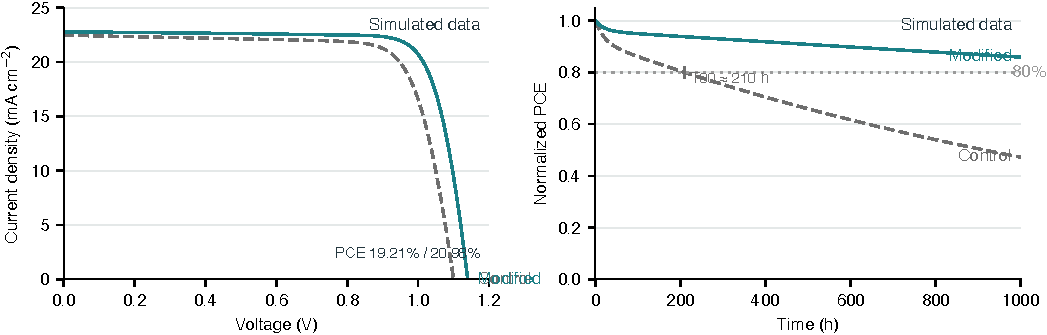
\includegraphics[width=\linewidth]{figures/ch09/ch09-05-data-panels-en.pdf}
\caption{The two data panels drawn at final size ($84 \times 56\ \text{mm}$ each). (c) Simulated $J\text{--}V$ curves for control (grey, dashed) and modified (teal, solid) devices. (d) Normalized PCE over time; the dotted line marks 80\%. The groups differ in both color and line style, so they remain distinguishable in greyscale. Curves were generated with a single-diode model and prescribed decay functions; simulated teaching data. Notice the lower-right corner of the left plot: when direct labels are anchored mechanically to the final data point of each curve, the two traces dropping to zero at $V_{\text{oc}}$ cause ``Control'' and ``Modified'' to collide with each other and with the terminal tick label, an issue corrected in the final assembly (Figure~\ref{fig:ch09-07}).}\label{fig:ch09-05}
\end{figure}

\textbf{Fourth, replace boxed legends with direct curve labels---and audit the rendered plot for geometric text collisions.}
For two-curve plots, replacing an enclosed legend box with color-matched text labels beside the traces removes eye jumps between legend and data.

Yet direct labeling cannot be coded blindly as ``place the label at the last point \texttt{(x[-1], y[-1])}.'' Inspecting the actual image in Figure~\ref{fig:ch09-05} shows the collision caused by automatic endpoint anchoring: in the left plot (Panel \textbf{c}), both $J\text{--}V$ curves drop steeply on the right to intersect the horizontal axis ($J = 0$) at their open-circuit voltages ($1.100\ \text{V}$ and $1.140\ \text{V}$). Binding labels to the curve endpoints causes ``Control'' and ``Modified'' to pile directly on top of each other over the \texttt{1.2} tick mark at the lower right, while the ``PCE 19.21\% / 20.98\%'' summary string is sliced through by the dashed control curve. In the right plot (Panel \textbf{d}), ``Modified,'' ``80\%,'' and ``Control'' crowd the right ends of their trajectories at $1000\ \text{h}$, and ``$\text{T80} \approx 210\ \text{h}$'' sits directly across the dashed curve.

Thus, \textbf{direct labels must be placed intentionally inside open white bands beside the curves and checked at 200\% zoom}. In our final assembly (Figure~\ref{fig:ch09-07}), we move ``Modified'' and ``Control'' in Panel \textbf{c} to the open band left of the steep drop---at $(0.96\ \text{V},\ 15.5\ \text{mA cm}^{-2})$ and $(1.00\ \text{V},\ 5.0\ \text{mA cm}^{-2})$---and move the PCE summary to the lower-left corner $(0.03,\ 0.04)$; in Panel \textbf{d}, we place the labels in the open corridors above their curves with semi-transparent white backing pads, eliminating all overlaps.

\textbf{Fifth, standardize units and embed provenance declarations inside every panel.}
Delete standalone subplot titles (``J-V curve,'' ``Stability test'') that repeat the caption; unify units to $\text{V}$, $\text{mA cm}^{-2}$, and $\text{h}$ with proper subscripts ($\mathrm{SnO_2}$); and place ``Not to scale'' (\textbf{a}), ``Model-generated illustration, not a micrograph'' (\textbf{b}), and ``Simulated data'' (\textbf{c}, \textbf{d}) inside the frames so provenance stays attached if a panel is reused in slides or posters.

\section{Alignment, labels, and white space}

When assembling four panels onto a shared canvas, visual polish depends on three geometric details: coordinate spine alignment, panel lettering, and purposeful whitespace.

\textbf{First: align coordinate axis spine boxes, not outer image bounding boxes.}
Panel \textbf{c}'s vertical axis has two-digit integers (\texttt{0--25}) and a title with superscripts, whereas Panel \textbf{d}'s vertical axis has decimals (\texttt{0.0--1.0}). If both plots are exported with tight bounding boxes (\texttt{bbox\_inches='tight'}) and aligned by their left image edges, their differing label widths push the inner coordinate rectangles out of alignment.

Because readers track the drawn axis spines rather than invisible text margins, composite assembly should avoid elastic auto-layout (\texttt{tight\_layout}) and \textbf{fix exact millimeter coordinates for every panel frame on the canvas}. On the $174.0 \times 116.0\ \text{mm}$ canvas of our final figure (Figure~\ref{fig:ch09-07}), we reserve $13.0\ \text{mm}$ on the left for vertical axis labels and lock the left column (Panel \textbf{a} frame and Panel \textbf{c} spine box) to $x = 13.0\text{--}82.0\ \text{mm}$ (width $69.0\ \text{mm}$). After a $6.0\ \text{mm}$ column gap and a $13.0\ \text{mm}$ label corridor, the right column (Panel \textbf{b} frame and Panel \textbf{d} spine box) is locked to $x = 101.0\text{--}170.0\ \text{mm}$ (width $69.0\ \text{mm}$), leaving a $4.0\ \text{mm}$ right margin with terminal ticks ``1.2'' and ``1000'' right-aligned inward. Both bottom spine boxes sit at $y = 11.0\text{--}57.0\ \text{mm}$ (height $46.0\ \text{mm}$), verified by script assertions (\texttt{assert}).

\textbf{Second: keep panel letters uniform in style, position, and baseline in an outer white corridor.}
Four rules govern panel letters:
\begin{enumerate}
\item \textbf{Single style:} Follow journal conventions uniformly ($10\ \text{pt}$ TeX Gyre Heros Bold lowercase \textbf{a}--\textbf{d}, without parentheses or periods).
\item \textbf{Aligned left edges and row baselines:} Align \textbf{a}, \textbf{c} at $x = 13.0\ \text{mm}$ and \textbf{b}, \textbf{d} at $x = 101.0\ \text{mm}$; align upper-row (\textbf{a}, \textbf{b}) and lower-row (\textbf{c}, \textbf{d}) letters on shared horizontal baselines $1.0\ \text{mm}$ above each panel frame's top edge.
\item \textbf{Top safety strip:} Reserve $5.0\ \text{mm}$ of white space at the top of the canvas so upper-row letters are never clipped.
\item \textbf{Outside dark interiors:} Place letters in the outer white corridor so they never vanish against Panel \textbf{b}'s dark upper background.
\end{enumerate}

\textbf{Third: use whitespace to signal grouping, and preserve native image aspect ratios.}
Between-group spacing should exceed within-group spacing: we set the horizontal column gap to $6.0\ \text{mm}$ and the vertical gap between the upper explanatory row (\textbf{a}, \textbf{b}) and lower data row (\textbf{c}, \textbf{d}) to $8.0\ \text{mm}$. Image panels must never use non-uniform stretching (\texttt{aspect='auto'}): at $69.0\ \text{mm}$ column width, Panel \textbf{a} ($1586 \times 992\ \text{px}$) is naturally $43.2\ \text{mm}$ tall and Panel \textbf{b} ($1536 \times 1024\ \text{px}$) is $46.0\ \text{mm}$ tall. Aligning their top edges at $y = 111.0\ \text{mm}$ leaves a natural $2.8\ \text{mm}$ white strip below Panel \textbf{a} for the incident-light and ``Not to scale'' labels.

\section{Case: Figure 2 from cluttered to review-ready}

We now walk through the complete assembly of Figure 2 for our planar perovskite solar cell case study---from material inventory and drawing brief to base-image auditing, initial v1 diagnosis, v2 revision, and reproduction in \scidraw{} (sharing the simulated dataset used in Chapters 12 and 13).

\subsection*{Step 1: Inventorying materials and simulation parameters}

The teaching scenario compares planar regular (n-i-p) control devices against devices with an interfacial passivation layer between the perovskite absorber and hole-transport layer. From bottom to top, the stack is glass / FTO / $\text{SnO}_2$ (schematic thickness $\sim 30\ \text{nm}$) / perovskite ($\sim 500\ \text{nm}$) / passivation layer (modified group only, ultra-thin) / spiro-OMeTAD ($\sim 200\ \text{nm}$) / Au ($\sim 80\ \text{nm}$), illuminated through the glass. We do not specify a perovskite composition or passivating molecule, nor do we report real device data.

Among the four inputs, M1 (Panel \textbf{a} structure schematic) and M2 (Panel \textbf{b} SEM-style cross-sectional illustration) are generated as text-free base images; M3 (Panel \textbf{c} $J\text{--}V$ curves) is solved by bisection in $0.5\ \text{mV}$ steps from the single-diode equation $J = J_{\text{L}} - J_0[\exp((V + J R_{\text{s}})/(n V_{\text{T}})) - 1] - (V + J R_{\text{s}})/R_{\text{sh}}$ at $25\ ^\circ\text{C}$ ($V_{\text{T}} = 0.025693\ \text{V}$) under AM1.5G ($100\ \text{mW cm}^{-2}$) for a single scan direction without hysteresis; and M4 (Panel \textbf{d} stability over $0\text{--}1000\ \text{h}$ in $10\ \text{h}$ steps) follows the bi-exponential decay $y(t) = [1 - b(1 - e^{-t/20})]e^{-t/\tau}$ ($b = 0.08, \tau = 1500\ \text{h}$ for control; $b = 0.04, \tau = 9000\ \text{h}$ for modified). Each group has one representative simulated curve; parameters and metrics appear in Table~\ref{tab:ch09-sim}.

\begin{table}[htbp]\centering\footnotesize
\setlength{\tabcolsep}{3.5pt}
\renewcommand{\arraystretch}{1.15}
\caption{Single-diode simulation parameters and derived photovoltaic metrics for panels c and d (simulated teaching data).}\label{tab:ch09-sim}
\begin{tabularx}{\linewidth}{@{}lcccYY@{}}
\toprule
\textbf{Group} & $J_{\text{L}}$ / target $V_{\text{oc}}$ & $n$ & $R_{\text{s}}$ / $R_{\text{sh}}$ ($\Omega\cdot\text{cm}^2$) & \textbf{Derived $J_{\text{sc}}$ / $V_{\text{oc}}$ / FF} & \textbf{Derived PCE and $T_{80}$} \\
\midrule
Control & $22.5\ \text{mA cm}^{-2}$ / $1.10\ \text{V}$ & 1.6 & $2.5$ / $1500$ & $22.46\ \text{mA cm}^{-2}$ / $1.100\ \text{V}$ / $0.777$ & $19.21\%$; $T_{80} = 210\ \text{h}$ \\
Modified & $22.8\ \text{mA cm}^{-2}$ / $1.14\ \text{V}$ & 1.5 & $2.0$ / $3000$ & $22.78\ \text{mA cm}^{-2}$ / $1.140\ \text{V}$ / $0.808$ & $20.98\%$; $T_{80} > 1000\ \text{h}$ \\
\bottomrule
\end{tabularx}
\end{table}

\begin{BookNote}
\textbf{Why not use an open-licensed real SEM micrograph for panel b?} Open-access literature provides CC BY 4.0 perovskite SEM images, such as Figure 6 of Burkitt, Searle, and Watson (2018) (top-view Jeol JSM-7800F SEM images of spin- and slot-die-coated films with $10\ \mu\text{m}$ and $1\ \mu\text{m}$ scale bars). However, that study uses a \textbf{mesoporous $\text{TiO}_2$ scaffold with $\text{MAPbI}_{3-x}\text{Cl}_x$ and $\sim 7\%$ stabilized efficiency}, unrelated to our planar $\text{SnO}_2$ stack and simulated metrics. Placing it into Figure 2 would falsely imply that the morphology and performance curves came from the same devices---violating Chapter 8's rule against presenting images from different samples as one source. Thus Panel \textbf{b} uses an explicitly labeled model-generated illustration; in real research, it must be an actual SEM image of the same device batch with raw files preserved.
\end{BookNote}

\subsection*{Step 2: The multi-panel drawing brief}

The complete drawing brief is written and saved in our own document; at layout time we choose ``Multi-panel figure'' in the \scidraw{} figure workflow guide (\sdtool{figure-workflow}) and follow the route into the panel tool, working from this brief:

\begin{Prompt}
[Use and audience] Paper Figure 2, double-column width 174 mm, height <= 120 mm;
audience is perovskite photovoltaics peers. Prepared to Springer-style standards:
minimum text >= 8 pt (verify current author instructions before submission).
[Main question] Does interface passivation raise both initial efficiency and stability?
[Panel roles]
a Device structure (modified stack; passivation highlighted) -- answers "what changed".
b Cross-section morphology -- answers "layer continuity". In this book, a model-generated
  illustration labeled in-panel "Model-generated illustration, not a micrograph".
c J-V curves (control, modified) -- answers "initial efficiency gain and driving parameter".
d Normalized PCE over time (control, modified, 0.8 line) -- answers "stability gain".
Reading order a->b->c->d: structure and morphology first, performance second.
[Layout] Top row a, b (explanatory); bottom row c, d (data); c and d axis boxes aligned
with identical height; 6 mm column gap; panel letters top-left, bold lowercase, shared baseline.
[Unified style] Single sans-serif font; ticks, axis titles, callouts 8 pt; panel letters
10 pt bold; axis lines 0.6 pt, data lines 1.2 pt; control #6E6E6E dashed, modified #1B7F86
solid; passivation layer in a also #1B7F86; 0.8 reference line light-grey dotted; direct
labels without legend boxes; units written V, mA cm^-2, h.
[Invariants] All numbers in c, d from the sim-perovskite dataset; aspect ratio of b locked;
in-panel notes "Simulated data" on c, d and "Not to scale" on a.
[Deliverables & acceptance] Vector PDF (selectable text) + high-res raster; processing log;
author-completed legend. At 174 mm (100% scale): min text >= 8 pt; c/d spines aligned;
greyscale distinguishable; b unstretched; all in-panel provenance notes visible.
\end{Prompt}

\subsection*{Step 3: Generating base images for panels a and b and auditing model deviations}

Panel \textbf{a}'s text-free base image is generated with the following English prompt (reserving the right 35\% of the canvas for labels):

\begin{Prompt}
A clean, flat, two-dimensional scientific schematic of a planar thin-film solar
cell shown as a stack of horizontal layers in side view with a slight sense of
thickness. From bottom to top: a thick pale blue-grey translucent glass slab;
a thin light grey conductive layer; a very thin off-white layer; a thicker
dark reddish-brown absorber layer; an extremely thin teal layer (hex #1B7F86)
directly on top of the absorber; a pale yellow layer; and a thin gold metal
layer on top. Three simple upward-pointing light arrows below the glass,
pale yellow with grey outline. The stack occupies the left 65% of the canvas;
leave the right 35% empty white space for labels added later.
White background, vector illustration style, no gradients, no shadows,
no 3D rendering, no glow, no texture. Layers are not to scale but each layer is
clearly separated by a thin dark grey outline.
Absolutely no text, no letters, no numbers, no labels, no symbols, no scale bar.
Aspect ratio 16:10.
\end{Prompt}

Running the prompt three times yields $1586 \times 992\ \text{px}$ PNGs (aspect ratio $1.599:1$, $-0.08\%$ from $16:10$), all showing the seven layers in order, three upward light arrows, and a text-free white background. However, candidate 2 draws the teal passivation layer too thick ($\sim 29\ \text{px}$), and candidate 3 shifts the teal toward a lighter cyan (median \texttt{\#298F97}) while widening the right margin to 38.5\%. Candidate 1 leaves 35\% whitespace on the right and renders a thin teal layer whose measured median color (\texttt{\#20868D}) is within $5\text{--}7$ RGB units of \texttt{\#1B7F86}, so we select it as the main base image. Two minor deviations remain: subtle shading and fine grain appear inside the layers despite \texttt{no gradients, no texture}, and the front glass layer ($\sim 148\ \text{px}$) is slightly thinner than the absorber layer ($\sim 158\ \text{px}$). We overlay the seven layer names with leader lines and add ``Not to scale'' at the bottom right (Figure~\ref{fig:ch09-03}).

\begin{figure}[htbp]\centering
\begin{tikzpicture}
\node[anchor=south west,inner sep=0] (img) at (0,0) {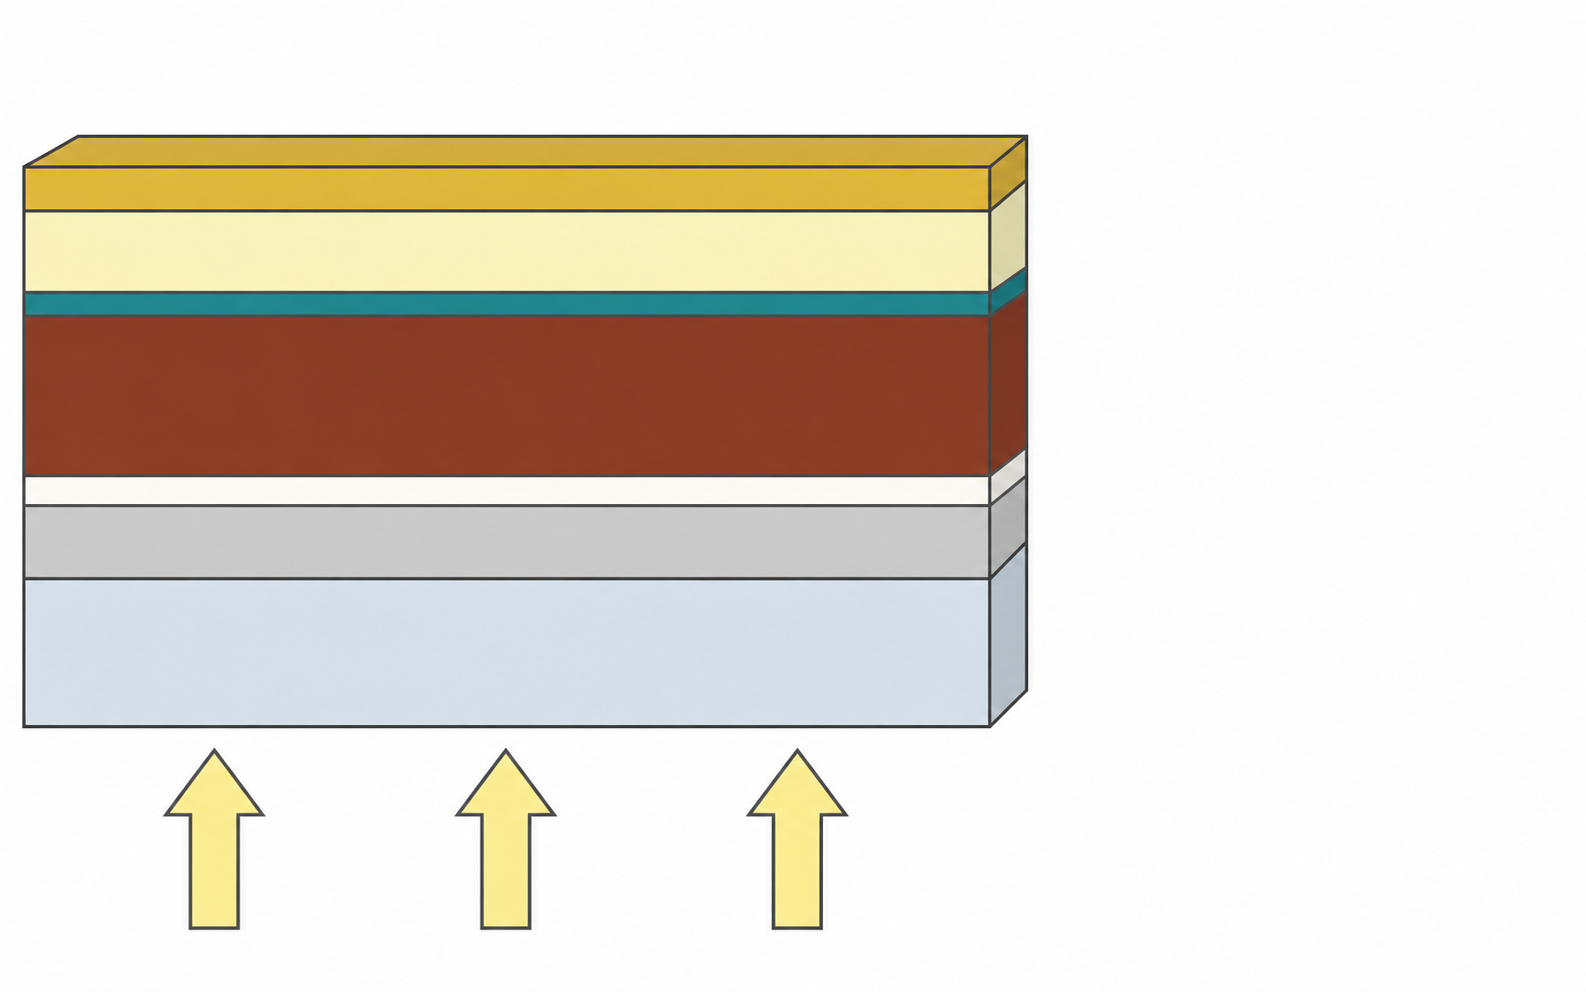
\includegraphics[width=0.86\linewidth]{figures/ch09/ch09-03-device-structure-base.png}};
\begin{scope}[x={(img.south east)},y={(img.north west)},font=\sffamily\footnotesize]
  \draw[BookInk!65,thin] (0.60,0.83) -- (0.69,0.86);
  \draw[BookInk!65,thin] (0.60,0.75) -- (0.69,0.76);
  \draw[BookTeal,thin] (0.60,0.698) -- (0.69,0.67);
  \draw[BookInk!65,thin] (0.60,0.60) -- (0.69,0.56);
  \draw[BookInk!65,thin] (0.60,0.505) -- (0.69,0.45);
  \draw[BookInk!65,thin] (0.60,0.45) -- (0.69,0.39);
  \draw[BookInk!65,thin] (0.60,0.33) -- (0.69,0.25);
  \node[anchor=west] at (0.70,0.86) {Au};
  \node[anchor=west] at (0.70,0.76) {spiro-OMeTAD};
  \node[anchor=west,text=BookTeal,font=\sffamily\footnotesize\bfseries] at (0.70,0.67) {Passivation layer};
  \node[anchor=west] at (0.70,0.56) {Perovskite};
  \node[anchor=west] at (0.70,0.45) {$\mathrm{SnO_2}$};
  \node[anchor=west] at (0.70,0.39) {FTO};
  \node[anchor=west] at (0.70,0.25) {Glass};
  \node[anchor=west] at (0.30,0.05) {Light};
  \node[anchor=south east,text=BookInk!80] at (0.98,0.02) {Not to scale};
\end{scope}
\end{tikzpicture}
\caption{Schematic of the modified device (panel a). The base image was drawn by an image-generation model and the layer names were added afterwards. The passivation layer uses the same teal as the ``modified'' series in the data panels. Layers are not to scale.}\label{fig:ch09-03}
\end{figure}

Panel \textbf{b}'s base image is generated with the following prompt (explicitly forbidding scale bars and instrument banners because a model-generated illustration has no physical scale):

\begin{Prompt}
A grayscale illustration in the visual style of a cross-sectional scanning
electron micrograph of a layered thin film, for use as a clearly labelled
teaching illustration. From bottom to top: a thick smooth featureless layer
filling the bottom third; a very thin slightly brighter layer; a thicker layer
made of densely packed columnar grains with visible grain boundaries; a
smoother amorphous layer; and a thin bright layer at the top. Dark background
above the top layer. Slightly irregular fractured edge. Even illumination,
moderate contrast. No scale bar, no data bar, no measurement marks, no text,
no letters, no numbers, no labels, no watermark. Aspect ratio 3:2.
\end{Prompt}

All three runs produce $1536 \times 1024\ \text{px}$ images (exact $3:2$) with five clear strata and no pseudo-text or fake scale bars. Candidate 1 has overly deep inter-grain crevices; candidate 2 expands the bottom layer to $42\%\text{--}43\%$ of the height with a steep downward slope at the top right. Candidate 3 (chosen as our main image) shows natural top fracture contours and clear grain boundaries, though the bottom layer still occupies $38\%\text{--}39\%$ of the height (above one-third) with faint graininess, and the RGB channels differ by up to $10$ units per pixel rather than being strictly identical. We overlay a white badge in the lower-left corner reading ``Model-generated illustration, not a micrograph'' (Figure~\ref{fig:ch09-04}).

\begin{figure}[htbp]\centering
\begin{tikzpicture}
\node[anchor=south west,inner sep=0] (img) at (0,0) {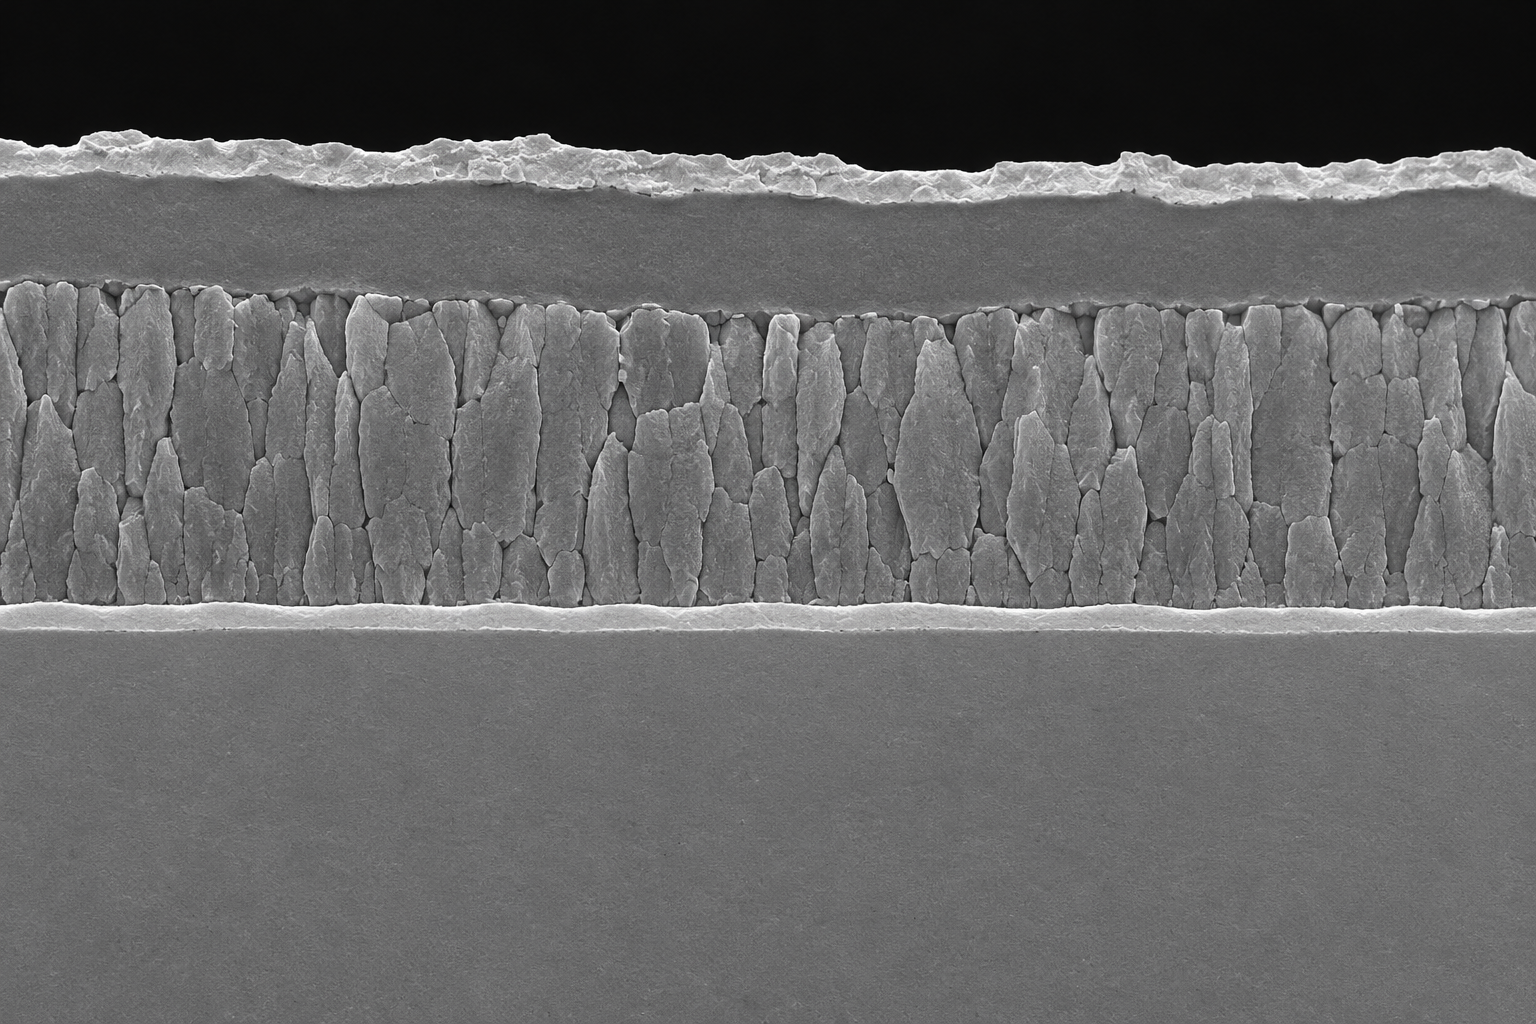
\includegraphics[width=0.78\linewidth]{figures/ch09/ch09-04-sem-like-illustration-base.png}};
\begin{scope}[x={(img.south east)},y={(img.north west)}]
  \node[anchor=south west,fill=white,fill opacity=0.90,text opacity=1,text=black,font=\sffamily\footnotesize,inner sep=2.5pt] at (0.02,0.03) {Model-generated illustration, not a micrograph};
\end{scope}
\end{tikzpicture}
\caption{Model-generated illustration of the cross-section (panel b). It was drawn by an image-generation model, is not a micrograph and has no physical scale; it only indicates layer order and layout. In a real paper this panel must be an actual SEM image of the same batch of devices, with the raw image and processing record kept (Chapter 8).}\label{fig:ch09-04}
\end{figure}

\subsection*{Step 4: Auditing the ten defects in the initial assembly (v1) and writing the revision order}

Figure~\ref{fig:ch09-06} reproduces the initial uncoordinated assembly (v1), with red badges 1--10 marking ten concrete defects on the canvas:

\begin{figure}[htbp]\centering
\resizebox{\linewidth}{!}{%
\begin{tikzpicture}
\definecolor{ChNineBad}{HTML}{C0392B}
\node[anchor=south west,inner sep=0] (img) at (0,0) {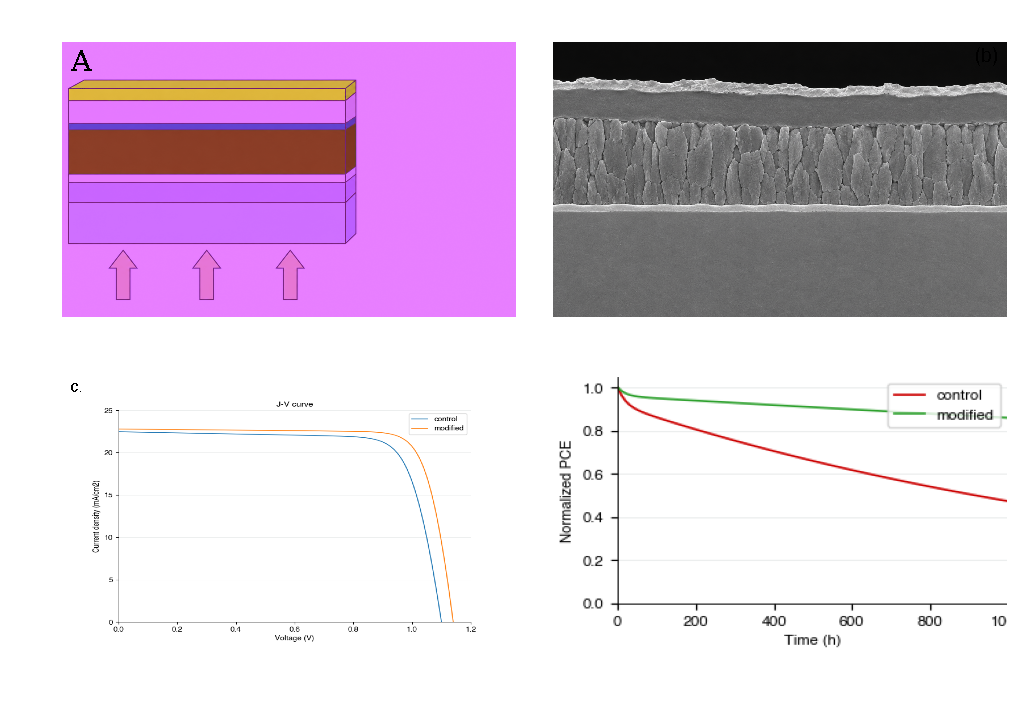
\includegraphics[width=\linewidth]{figures/ch09/ch09-06-assembly-v1-en.pdf}};
\begin{scope}[x={(img.south east)},y={(img.north west)}]
  \tikzset{
    badnum/.style={draw=white,line width=0.7pt,fill=ChNineBad,text=white,circle,font=\sffamily\bfseries\scriptsize,inner sep=1pt,minimum size=4.0mm},
    badtxt/.style={fill=white,fill opacity=0.88,text opacity=1,text=ChNineBad!90!black,font=\sffamily\scriptsize\bfseries,inner sep=1.2pt,rounded corners=1pt}
  }
  \node[badnum] (b1) at (0.03,0.95) {1};
  \node[badtxt,anchor=west] at (b1.east) {Mixed panel letters};
  \node[badnum] (b2) at (0.62,0.30) {2};
  \node[badtxt,anchor=west] at (b2.east) {Mismatched font sizes};
  \node[badnum] (b3) at (0.20,0.70) {3};
  \node[badtxt,anchor=west] at (b3.east) {Inconsistent color semantics};
  \node[badnum] (b4) at (0.85,0.20) {4};
  \node[badtxt,anchor=east] at (b4.west) {Indistinguishable in greyscale};
  \node[badnum] (b5) at (0.75,0.40) {5};
  \node[badtxt,anchor=west] at (b5.east) {Legend box overlaps curve};
  \node[badnum] (b6) at (0.50,0.08) {6};
  \node[badtxt,anchor=west] at (b6.east) {Misaligned axis boxes};
  \node[badnum] (b7) at (0.75,0.75) {7};
  \node[badtxt,anchor=west] at (b7.east) {Panel b stretched};
  \node[badnum] (b8) at (0.50,0.52) {8};
  \node[badtxt,anchor=west] at (b8.east) {Uneven panel spacing};
  \node[badnum] (b9) at (0.92,0.92) {9};
  \node[badtxt,anchor=east] at (b9.west) {Missing provenance notes};
  \node[badnum] (b10) at (0.30,0.45) {10};
  \node[badtxt,anchor=west] at (b10.east) {Redundant subplot titles};
\end{scope}
\end{tikzpicture}}
\caption{First assembly (v1, a deliberately reproduced counter-example). Numbers 1--10 mark the problems discussed in the text. Panel b is a model-generated illustration, not a micrograph, and panels c and d show simulated data; this version omits those in-panel notes, which is problem 9.}\label{fig:ch09-06}
\end{figure}

\begin{enumerate}
\item \textbf{Mixed and missing panel letters (1):} Panel \textbf{a} uses a $14\ \text{pt}$ serif ``A''; Panel \textbf{b} has a $9\ \text{pt}$ ``(b)'' nearly lost in the dark upper-right background; Panel \textbf{c} uses ``c.''; and Panel \textbf{d} omits its letter.
\item \textbf{Mismatched font sizes and clipped ticks (2):} Panel \textbf{c} was plotted at $8 \times 6\ \text{in}$ ($10\ \text{pt}$) and scaled down, shrinking its ticks to $\sim 4.5\ \text{pt}$; Panel \textbf{d} was plotted at $84 \times 56\ \text{mm}$ ($8\ \text{pt}$), and its rightmost tick ``1000'' is clipped to ``10'' at the border.
\item \textbf{Inconsistent color semantics (3):} A hue shift in Panel \textbf{a} turned the passivation layer deep purple and tinted the background magenta-violet; Panel \textbf{c} uses default blue/orange; and Panel \textbf{d} uses red/green.
\item \textbf{Indistinguishable in greyscale (4):} Both data panels use solid lines for both groups, and Panel \textbf{d}'s red/green pairing is unfriendly to color-blind readers.
\item \textbf{Legend box overlapping data (5):} Both data plots use boxed legends, and Panel \textbf{d}'s legend sits directly over the green modified curve.
\item \textbf{Misaligned axis spine boxes (6):} The coordinate spine boxes of \textbf{c} and \textbf{d} are offset by $1.4\ \text{mm}$ on the left edge and $3.2\ \text{mm}$ on the bottom edge.
\item \textbf{Stretched image panel (7):} Panel \textbf{b} uses \texttt{aspect='auto'} to match Panel \textbf{a}'s height, vertically distorting the grains.
\item \textbf{Uneven panel spacing (8):} Irregular \texttt{GridSpec} gaps obscure the grouping hierarchy.
\item \textbf{Missing provenance notes and benchmark line (9):} Panels lack ``Not to scale,'' ``Model-generated illustration,'' and ``Simulated data'' badges, Panel \textbf{a} has no layer names, and Panel \textbf{d} omits the $0.8$ line.
\item \textbf{Redundant subplot titles and unformatted units (10):} Panels \textbf{c} and \textbf{d} have top titles (``J-V curve,'' ``Stability test'') duplicating the legend, and Panel \textbf{c} writes \texttt{mA/cm2}.
\end{enumerate}

We address all ten issues with a structured revision order:

\begin{Prompt}
Revision order (v1 -> v2)
1. Unify panel letters to 10 pt bold sans-serif lowercase a-d outside each frame's top-left
   corner on shared row baselines (reserve a 5 mm white safety strip at the canvas top).
2. Redraw c and d directly on the 174 x 116 mm master canvas at 8 pt text (scale factor 1.0).
3. Unify color semantics: control #6E6E6E dashed, modified #1B7F86 solid; restore the clean
   white-background base image in a and set the "Passivation layer" label in #1B7F86.
4. Remove boxed legends; place color-matched direct labels ("Control", "Modified") in open
   white bands beside the curves so no text touches a data trace or tick mark.
5. Lock horizontal frame spans: left column (a, c) x = 13-82 mm; right column (b, d)
   x = 101-170 mm; c and d spine boxes at y = 11-57 mm (46 mm tall); right-align terminal
   ticks "1.2" and "1000" inside the 4 mm right margin.
6. Place a and b at native aspect ratios (69 x 43.2 mm and 69 x 46.0 mm), top-aligned at y = 111 mm.
7. Set inter-column gap to 6 mm (plus 13 mm y-axis corridor) and inter-row gap to 8 mm.
8. Add "Simulated data" to c and d, "Model-generated illustration, not a micrograph" to b,
   layer labels + "Not to scale" to a, and the 0.8 dotted line + "80%" + "T80 ~ 210 h" to d.
9. Remove subplot titles; standardize units to V, mA cm^-2, and h.
10. Export vector PDF (pdf.fonttype = 42) and 300 dpi PNG; log panel dimensions and scale factors.
\end{Prompt}

\subsection*{Step 5: Revised assembly (v2) and reproducing the layout in SciDraw AI}

The revised composite figure (v2) appears in Figure~\ref{fig:ch09-07}. To assemble the same four pre-rendered panels in the \scidraw{} multi-panel tool (\sdtool{multi-panel-figure-maker}), follow three checkpoints:

\begin{figure}[htbp]\centering
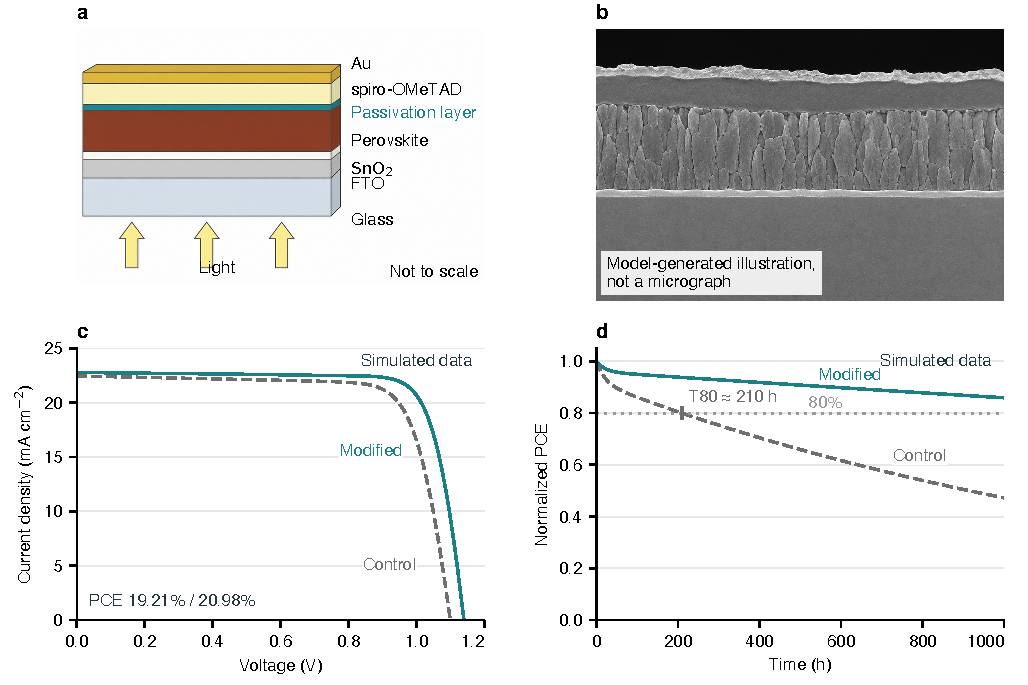
\includegraphics[width=\linewidth]{figures/ch09/ch09-07-assembly-final-en.pdf}
\caption{Revised assembly (v2). \textbf{Fig.~2 | Effect of interface passivation on the initial performance and operational stability of perovskite solar cells (simulated teaching data).} \textbf{a}, Schematic of the modified device (glass/FTO/$\text{SnO}_2$/perovskite/passivation layer/spiro-OMeTAD/Au; light enters through the glass); the control device has no passivation layer; layer thicknesses are not to scale. \textbf{b}, Illustration of the cross-section drawn by an image-generation model; \textbf{not a micrograph}, shown only to indicate layer order. \textbf{c}, $J\text{--}V$ curves of control (grey, dashed) and modified (teal, solid) devices simulated with a single-diode model (AM1.5G, $100\ \text{mW cm}^{-2}$, one scan direction, no hysteresis modeled); PCE 19.21\% (control) and 20.98\% (modified). \textbf{d}, Normalized PCE over time under simulated conditions (continuous 1-sun illumination, maximum-power-point tracking, $\text{N}_2$, about $25\ ^\circ\text{C}$); the dotted line marks 80\% of the initial value; $T_{80}$ is about $210\ \text{h}$ for the control, and the modified device stays above 80\% for $1{,}000\ \text{h}$. Panels c and d show one simulated curve per group, not a distribution across devices, and no statistical test was performed. Simulation parameters and script are provided in the book repository.}\label{fig:ch09-07}
\end{figure}

\begin{enumerate}
\item \textbf{File handoff and journal presets:} Tools do not transfer images automatically; upload the labeled PNGs for \textbf{a} and \textbf{b} and final-size PNGs for \textbf{c} and \textbf{d} into \texttt{/multi-panel-\allowbreak figure-\allowbreak maker} (saved in browser local storage). Choose the Springer or Cell $174\ \text{mm}$ double-column preset and a $2 \times 2$ grid with auto-numbering. Because numbering follows the preset (lowercase \textbf{a} for Springer, uppercase \textbf{A} for Cell), verify the target journal's author instructions before submission.
\item \textbf{Export bundle and tool boundaries:} Export the ZIP containing TIFF, PNG, PDF, PPTX, and the processing record. In PPTX, panel bitmaps and outer letters are separate objects, but text inside panel bitmaps is not editable; the tool does not auto-plan layouts, edit internal panel text, or vectorize bitmaps.
\item \textbf{Reading the processing record for font size and resolution:} Check the logged cell dimensions and scale factors. If Panel \textbf{c} was plotted at $84\ \text{mm}$ ($8\ \text{pt}$) but placed at $80\ \text{mm}$ (scale factor $0.952$), its effective font size drops to $8 \times 80 / 84 \approx 7.6\ \text{pt}$, requiring re-export from the script at the exact cell width. Bitmap resolution equals source pixel width divided by placed width in inches: at $69.0\ \text{mm}$ ($2.717\ \text{in}$), Panel \textbf{a} ($1586\ \text{px}$) and Panel \textbf{b} ($1536\ \text{px}$) reach $1586 / 2.717 \approx 584\ \text{ppi}$ and $1536 / 2.717 \approx 565\ \text{ppi}$, well above $300\ \text{ppi}$.
\end{enumerate}

\section{Legends: AI drafts, the author completes}

A complete multi-panel legend contains five parts: an opening title sentence, panel-by-panel descriptions (defining visual encodings), key experimental or simulation conditions, sample sizes and statistical methods, and data provenance declarations.

When you upload the composite PNG to the \scidraw{} legend assistant (\sdtool{figure-legend}), the tool reads only the image pixels and outputs a 40--120 word descriptive draft, typically along the lines of: ``Device structure, cross-sectional morphology, and photovoltaic performance of perovskite solar cells. (a) Schematic of the layered device architecture. (b) Cross-sectional image of the device stack. (c) $J\text{--}V$ curves of control and modified devices. (d) Normalized PCE as a function of time.''

By design, \sdtool{figure-legend} never fabricates sample sizes, $p$-values, statistical tests, test conditions, or chemical formulas invisible in the image. The author must separate \textbf{what is visible in the pixels} from \textbf{what the author must supply} (Figure~\ref{fig:ch09-08}):

\begin{figure}[htbp]\centering
\resizebox{\linewidth}{!}{% FIG ch09-08 legend drafting (English)
\begin{tikzpicture}[
  x=1mm, y=1mm,
  font=\sffamily\scriptsize,
  text=BookInk,
  col/.style={draw=BookInk!45, line width=0.4pt, rounded corners=1pt, inner sep=2mm, align=justify, text width=78mm},
  hi/.style={fill=BookPale, draw=BookTeal, line width=0.8pt, rounded corners=1pt, inner sep=1.5mm},
  tag/.style={font=\tiny\bfseries, text=BookTeal, anchor=east},
]
  \node[font=\small\bfseries, anchor=west] at (0, 118) {Legend drafting checklist};
  \node[col, anchor=north west] at (0, 112) {
    \textbf{/figure-legend draft (verbatim)}\par\vspace{1mm}
    \fbox{\parbox[t]{72mm}{\centering Pending measurement; see \texttt{provenance/ch09/figure-legend-draft-en.txt}}}
  };
  \node[col, anchor=north west] at (88, 112) {
    \textbf{Author-completed (excerpt)}\par\vspace{1mm}
    \tikz{\node[hi, text width=72mm, anchor=west] at (0,0) {
      \textbf{Fig.~2 |} Effect of interface passivation \ldots\ (\textbf{simulated teaching data}).
    }; \node[tag] at (-1,0) {[data]};}\par
    \tikz{\node[hi, text width=72mm, anchor=west] at (0,0) {
      \textbf{b}, illustration drawn by an image-generation model; \textbf{not a micrograph} \ldots
    }; \node[tag] at (-1,0) {[definition]};}\par
    \tikz{\node[hi, text width=72mm, anchor=west] at (0,0) {
      Panels c and d: one simulated curve per group; no statistical test; see \texttt{sim\_perovskite.py}.
    }; \node[tag] at (-1,0) {[source]};}
  };
  \node[anchor=west, text=BookInk!70] at (0, 4) {
    Correction: \sout{cross-section image} $\rightarrow$ model-generated illustration, not a micrograph
  };
\end{tikzpicture}
}
\caption{AI drafts the legend; the author completes it. Left: the draft produced by \sdtool{figure-legend} from the image (verbatim). Right: the completed legend; highlighted text is information that cannot be seen in the image and must come from the author.}\label{fig:ch09-08}
\end{figure}

\begin{itemize}
\item \textbf{Correcting visual misclassifications:} The draft may call Panel \textbf{b} a ``cross-sectional image / SEM image''; replace this with ``Illustration of the cross-section drawn by an image-generation model; not a micrograph, shown only to indicate layer order.''
\item \textbf{Supplying five categories of context:} (1) \textbf{[Data nature]} Simulated teaching data, layers not to scale, not a micrograph; (2) \textbf{[Devices and conditions]} Seven-layer stack and illumination side, single-diode model (AM1.5G, $100\ \text{mW cm}^{-2}$, one scan direction, no hysteresis---real perovskite cells exhibit hysteresis and require reporting scan direction and rate per Snaith et al., 2014), and stability conditions (continuous 1-sun illumination, MPP tracking, $\text{N}_2$, $\sim 25\ ^\circ\text{C}$; verify any ISOS-L-1 protocol label against Khenkin et al., 2020); (3) \textbf{[Samples and statistics]} PCE $19.21\%$ vs.\ $20.98\%$, stating that each curve is a single simulated trajectory with no device distribution or statistical test; (4) \textbf{[Definitions]} Dotted line at 80\% of initial efficiency, control $T_{80} \approx 210\ \text{h}$, modified $> 1000\ \text{h}$; (5) \textbf{[Source]} Simulation parameters and script location (see full caption in Figure~\ref{fig:ch09-07}).
\end{itemize}

For empirical research papers, authors can fill in the following template from their lab records:

\begin{BookNote}
\textbf{Empirical paper legend template:} \textbf{c}, Representative $J\text{--}V$ curves (reverse scan, [scan rate] $\text{mV s}^{-1}$, active area [area] $\text{cm}^2$, aperture mask [with/without]); inset table gives photovoltaic parameters (mean $\pm$ s.d.) for $n =$ [devices] devices across [batches] independent batches. \textbf{d}, Normalized PCE of $n =$ [devices] unencapsulated devices per group under [atmosphere] at [temperature] $^\circ\text{C}$; shaded bands show [s.d.\ / s.e.m.\ / range]; $T_{80}$ is defined as [time to first drop below 80\% / fitted value]. Statistical test: [method], [$P$ value].
\end{BookNote}

Before delivery, combine \sdtool{figure-checker} with script assertions to complete the eight-point verification in Table~\ref{tab:ch09-verify}.

\begin{table}[htbp]\centering\footnotesize
\setlength{\tabcolsep}{3pt}
\renewcommand{\arraystretch}{1.15}
\caption{Eight-point pre-delivery verification of the final composite figure (Figure~\ref{fig:ch09-07}).}\label{tab:ch09-verify}
\begin{tabularx}{\linewidth}{@{}>{\raggedright\arraybackslash}p{26mm}YY@{}}
\toprule
\textbf{Check item} & \textbf{Verification method} & \textbf{Measured result on final figure} \\
\midrule
Numerical consistency & Script assertions comparing summary CSV metrics against plot and caption numbers & PCE ($19.21\%$ / $20.98\%$) and $T_{80}$ ($210\ \text{h}$ / $>1000\ \text{h}$) match identically \\
100\% print font size & Check PDF font properties at $174\ \text{mm}$ width or measure cap height ($8\ \text{pt} \approx 2.0\ \text{mm}$) & Panel letters $10\ \text{pt}$ bold; all other text $8\ \text{pt}$ with zero border clipping \\
Spine box alignment & Assert millimeter coordinates of all four frames via \texttt{ax.get\_position()} & \textbf{a}/\textbf{c} locked to $13\text{--}82\ \text{mm}$; \textbf{b}/\textbf{d} locked to $101\text{--}170\ \text{mm}$; \textbf{c}/\textbf{d} bottom at $11\ \text{mm}$ \\
Image aspect ratio & Compare placed frame ratios against source PNG pixel dimensions & Panel \textbf{a} ($69.0 \times 43.2\ \text{mm}$) and Panel \textbf{b} ($69.0 \times 46.0\ \text{mm}$) error $< 0.1\%$ \\
Greyscale \& CVD safety & Greyscale conversion and Machado (2009) CVD simulation / \sdtool{figure-checker} & Grey dashed, teal solid, and light-grey dotted lines remain separable \\
In-panel declarations & Visual audit of all four panel interiors at 100\% scale & ``Not to scale,'' ``Model-generated illustration, not a micrograph,'' and ``Simulated data'' visible \\
Scale factor \& ppi & Check processing log scale factor and compute source pixels $\div$ placed inches & \textbf{c}, \textbf{d} scale factor $1.0$; \textbf{a} $\sim 584\ \text{ppi}$, \textbf{b} $\sim 565\ \text{ppi}$ \\
Legend traceability & Cross-check every number and condition in the caption against data and script settings & All numbers trace to data files and simulation parameters; no unsupported claims \\
\bottomrule
\end{tabularx}
\end{table}

\section{What AI Can and Cannot Do at This Stage}

Table~\ref{tab:ch09-01} summarizes the responsibilities of AI, deterministic tools, and the author across multi-panel assembly and legend preparation.

\begin{table}[htbp]\centering\footnotesize
\setlength{\tabcolsep}{3pt}
\renewcommand{\arraystretch}{1.15}
\caption{What AI can do, what AI cannot do, and what the author must verify when assembling multi-panel figures.}\label{tab:ch09-01}
\begin{tabularx}{\linewidth}{@{}>{\raggedright\arraybackslash}p{20mm}YYY@{}}
\toprule
\textbf{Stage} & \textbf{What AI can do} & \textbf{What AI cannot do} & \textbf{What the author must verify} \\
\midrule
Panel roles & List candidate panel roles and reading orders from a brief; flag panels unrelated to the main question & Judge whether evidence suffices to support the conclusion, or decide which data may be omitted & The sub-question each panel answers; destination of removed panels (Supplementary Information) \\
Grid planning & Convert journal widths into cell sizes; write \texttt{gridspec} or fixed-axis scripts & Weigh scientific importance to allocate area (the multi-panel tool does not do AI layout planning) & Final dimensions, preserved aspect ratios, and grouping whitespace \\
Schematic panels & Generate text-free base images showing layer order or stylized morphology & Guarantee accurate layer sequence, realistic proportions, or empirical morphological evidence & Layer count and sequence, shared color semantics, and ``not to scale / model-generated'' labels \\
Data panels & Write plotting scripts to spec; unify \texttt{rcParams} & Select or alter data values, or invent error bands that do not exist & Values match data files; font size meets specs at final width; greyscale separability \\
Layout \& export & \scidraw{} multi-panel tool: grids, row/column spans, auto-numbering, journal presets, processing logs, TIFF/PNG/PDF/PPTX & Edit text inside panel bitmaps, unify fonts across rasterized panels, or turn bitmaps into editable vectors & Scale factors and effective ppi in the processing record; numbering style matches journal rules \\
Figure legend & \sdtool{figure-legend}: draft descriptions of visually observable features & Write sample sizes, batches, test conditions, statistical methods, or data nature (never fabricated by design) & Supply $n$, conditions, statistics, definitions ($T_{80}$), and sources; remove misclassifications (e.g., SEM) \\
Technical check & \sdtool{figure-checker}: check format, resolution, greyscale, and color-vision risks & Audit scientific conclusions or statistical choices & Full scientific verification beyond technical checks \\
\bottomrule
\end{tabularx}
\end{table}

\section{Chapter Checklist}

\begin{itemize}
\item The main question of the composite figure is written down, every panel has a clear sub-question or evidential role, and unrelated panels have been moved out.
\item The canvas is set to the target journal's final width ($174\ \text{mm}$ in this example) and stays within height limits.
\item Data panels are exported directly at their final cell dimensions with an assembly scale factor of $1.0$ (or effective font sizes have been calculated from the scale factor).
\item One sans-serif font family is used throughout; minimum text meets journal rules; panel letters share a uniform style, size, and position.
\item Coordinate axis spine boxes of side-by-side data panels are aligned; inter-panel gaps are uniform, with between-group whitespace larger than within-group whitespace.
\item Each experimental group keeps the same color across all panels; line styles or direct labels provide non-color redundancy; greyscale and color-vision checks pass.
\item Image panels preserve their native aspect ratios without stretching.
\item Declarations for simulated data, model-generated illustrations, and not-to-scale schematics are written \textbf{inside the panels} as well as in the legend.
\item The legend includes a title sentence, panel-by-panel descriptions, sample sizes and replicates, test conditions, statistical methods and error definitions, threshold definitions (such as $T_{80}$), and data/code sources.
\item Processing records, scripts, raw data, and exported composite files are archived together, with file handoffs between scripts and layout tools recorded.
\end{itemize}

\section{Exercises}

\begin{enumerate}
\item \textbf{Panel argument mapping (pen and paper).} Take one of your recent multi-panel figures, write down its main question and the sub-question for each panel, and identify one panel that does not directly answer the main question. Explain whether it should stay, be merged, or move to the Supplementary Information.
\item \textbf{Final-size check (script).} Using this chapter's data-panel plotting script, export Panel \textbf{c} both at $\text{figsize}=(8,6)\ \text{in}$ and at $84 \times 56\ \text{mm}$, place each into an $84\ \text{mm}$-wide cell, and calculate the effective printed tick-label font size in both cases; then change the control curve to a solid line matching the modified curve, convert to greyscale, and record whether the groups can be distinguished.
\item \textbf{Hands-on practice with \scidraw{}.} Import the four panel PNGs provided with this chapter into \texttt{/multi-panel-\allowbreak figure-\allowbreak maker}, select the Springer and Cell $174\ \text{mm}$ presets in turn, and compare their numbering styles; export the ZIP archive, read Panel \textbf{c}'s scale factor from the processing record, and compute its effective font size. Next, upload the exported PNG to \sdtool{figure-legend}, save the verbatim draft, and complete the legend across the categories in Section 9.6. \emph{Extension:} Read Figure 6 of Burkitt et al.\ (2018) (CC BY 4.0, real SEM figure), list the information a real SEM panel must provide inside the figure and in the legend (instrument, viewing angle, scale bar, sample stack, and processing), and explain why it cannot be placed into Figure 2 of this chapter.
\end{enumerate}

\section*{References}

\begin{itemize}
\item Burkitt D, Searle J, Watson T. Perovskite solar cells in N-I-P structure with four slot-die-coated layers. \textit{Royal Society Open Science}. 2018;5(5):172158. doi:10.1098/\allowbreak rsos.172158
\item Crameri F, Shephard GE, Heron PJ. The misuse of colour in science communication. \textit{Nature Communications}. 2020;11:5444. doi:10.1038/\allowbreak s41467-020-19160-7
\item Jambor H, Antonietti A, Alicea B, et al. Creating clear and informative image-based figures for scientific publications. \textit{PLOS Biology}. 2021;19(3):e3001161. doi:10.1371/\allowbreak journal.pbio.3001161
\item Khenkin MV, Katz EA, Abate A, et al. Consensus statement for stability assessment and reporting for perovskite photovoltaics based on ISOS procedures. \textit{Nature Energy}. 2020;5(1):35--49. doi:10.1038/\allowbreak s41560-019-0529-5
\item Kojima A, Teshima K, Shirai Y, Miyasaka T. Organometal halide perovskites as visible-light sensitizers for photovoltaic cells. \textit{Journal of the American Chemical Society}. 2009;131(17):6050--6051. doi:10.1021/\allowbreak ja809598r
\item Machado GM, Oliveira MM, Fernandes LAF. A physiologically-based model for simulation of color vision deficiency. \textit{IEEE Transactions on Visualization and Computer Graphics}. 2009;15(6):1291--1298. doi:10.1109/\allowbreak TVCG.2009.113
\item Nature Portfolio. Preparing figures -- our specifications. \url{https://research-figure-guide.nature.com/figures/preparing-figures-our-specifications/} (accessed 2026-10-29).
\item Rougier NP, Droettboom M, Bourne PE. Ten simple rules for better figures. \textit{PLoS Computational Biology}. 2014;10(9):e1003833. doi:10.1371/\allowbreak journal.pcbi.1003833
\item Snaith HJ, Abate A, Ball JM, et al. Anomalous hysteresis in perovskite solar cells. \textit{The Journal of Physical Chemistry Letters}. 2014;5(9):1511--1515. doi:10.1021/\allowbreak jz500113x
\item Wong B. Points of view: Color blindness. \textit{Nature Methods}. 2011;8(6):441. doi:10.1038/\allowbreak nmeth.1618
\end{itemize}

% TODO: provenance/ch09/figure-legend-draft-en.txt has not yet been generated (the left column of figures/ch09/ch09-08-legend-drafting-en.tex currently shows a "Pending measurement" placeholder box).
% TODO: standalone pre-overlaid bitmaps figures/ch09/ch09-03-device-structure-en.png and figures/ch09/ch09-04-sem-like-illustration-en.png have not been generated separately (this chapter displays the base images with TikZ overlays as specified by book-spec Section 6, and the composite figure ch09-07 embeds the overlays directly).
% TODO: figures/ch09/ch09-05-data-panels-en.pdf was exported before the direct-label coordinate adjustment in ch09_plot_utils.py (the "Control" and "Modified" labels at the lower right still overlap at the curve endpoints); re-running scripts/ch09_panels.py will synchronize it with ch09-07.
